\chapter{Megvalósítás}\label{ch:MEGVALOSITAS}
\begin{osszefoglal}
	A projekt egy EV3 készletből épített kétkerekű egyensúlyozó robot irányítását valósítja meg hálózaton keresztül, telefonos alkalmazáson segítségével. E fejezet alatt bemutatásra kerülnek a megvalósítás során felmerült problémák, ezek megoldása és a felhasznált technológiák.
\end{osszefoglal}

\section{EV3 programozása}\label{sec:MEGVALOSITAS:lejos}
A LEGO MINDSTORMS kifejlesztett egy programozási környezetet, mely célja, hogy a megépített robotot különböző funkcionalitásokkal lehessen felruházni. E környezet lehetővé teszi a kisebb korosztály számára is a robotok programozását. Különböző grafikus elemekből úgynevezett blokkokból épül fel a program, amely USB-n keresztül kitelepíthető az EV3 vezérlőegységen futó LEGO MINDSTORMS által fejlesztett firmware.
Az előbb említett programozási környezet nem alkalmas komplexebb problémák megoldására. Ezért több firmware-t is kifejlesztettek melyek magas szintű programozási nyelveket támogatnak. Esetünkben a leJOS firmware-t használjuk.

A leJOS firmware-t José Solórzano hozta létre 1999 végén és azóta is folyamatosan fejlesztik. Linux alapú, nyílt forráskódú, magába foglalja a JVM-t (Java virtual machine), a neve is rámutat a Java programozhatóságra JOS(Java Operating System). Lehetővé teszi, a robot programozását Java-ban, támogatja a objektum orientált programozást. Mindezek lehetővé teszik a socket alapú komunikációt, szinkronizálhatóságot, szálak alkalmazását és Java típusok használatát. A leJOS hozzáférést biztosít az EV3 vezérlőegységen levő portokhoz, ezáltal kezelhetjük a giroszkóp szenzort (\ref{gyroPort} ábra) illetve a nagy motorokat (\ref{motorPort} ábra). Elrejti a szenzorok implementációját, lehetővé téve a magas szintű absztrakció használatát.

\begin{lstlisting}[label=motorPort, caption= Az \texttt{A} porton keresztül hozzáférés a motorhoz, language=Java]

EncoderMotor motor = new UnregulatedMotor(MotorPort.A);

\end{lstlisting}

\begin{lstlisting}[label=gyroPort, caption= Az \texttt{S2} porton keresztük hozzáférés a giroszkop szenzorhoz, language=Java]

EV3GyroSensor gyroSensor =  new EV3GyroSensor(SensorPort.S2);

\end{lstlisting}

A \ref{gyroRateMod} és a \ref{gyroAngleMod} ábrákon látható a leJOS firmware által biztosított két mód, a giroszkóp szenzor használatához. A \texttt{rate} mód a szögsebességet méri, amelyet szög/másodperce -ben kapunk meg. A \ref{gyroRateMod} ábrán látható a mód kiválasztása és ezt követően a mintavételezés, melynek eredménye a \texttt{sample} tömb első eleme lesz. Használható \texttt{angle} módban is, amely \ref{gyroAngleMod} ábrán látható. E mód a szenzor kezdő orientációjához képest mér. Mintavételezés hasonlóan történik, mint az előbb említett módnál, annyi különbséggel hogy ez esetben szöget mér a kezdő pozíciójához képest. Mindkét mód esetében a \texttt{reset} metódus hívással újra kalibrálhatjuk a szenzort.

\begin{lstlisting}[label=gyroRateMod, caption= Giroszkóp szenzor \texttt{rate} mód használata, language=Java]

float[] sample = new float[1];
EV3GyroSensor gyroSensor =  new EV3GyroSensor(SensorPort.S2);

SampleProvider gyroMode = gyroSensor.getRateMode();

gyro.fetchSample(sample, 0);

\end{lstlisting}

\begin{lstlisting}[label=gyroAngleMod, caption= Giroszkóp szenzor \texttt{angle} mód használata, language=Java]

float[] sample = new float[1];
EV3GyroSensor gyroSensor =  new EV3GyroSensor(SensorPort.S2);

SampleProvider gyroMode = gyroSensor.getAngleMode();

gyro.fetchSample(sample, 0);

\end{lstlisting}

A nagy motorok esetében is két módot biztosít a leJOS firmware, amelyek a \ref{motorUnregMod} és \ref{motorRegMod} ábrán láthatóak. Rendre értelemszerűen a nem szabályzott és a szabályzott módok. 

A motor nem szabályzott mód (\ref{motorUnregMod} ábra) használata esetén az irányítást a \texttt{setPower} metódus hívással valósítjuk meg, amelynek ha az átadott érték pozitív akkor előre forog illetve ha negatív akkor hátra. A \texttt{resetTachoCount} valamint \texttt{getTachoCount} metódusokkal kezeljük a motorban levő forgás mérő szenzort, melynek számlálójának értékét lekérhetjük vagy lenullázhatjuk. Esetünkbe szükséges a pozíció illetve a sebesség meghatározása, e megvalósítását az előbb említett metódus teszi lehetővé. Az eltelt idő, a kerék sugara és a fordulat szám segítségével, amelyet \texttt{getTachoCount} térit vissza, kiszámítható a robot sebessége valamint a pozíciója. A \texttt{stop} metódus hívása esetén a motor blokkolt állapotba kerül.    

A motor szabályzott mód (\ref{motorRegMod} ábra) esetén némely funkcionalitás eltér az előbb említett módhoz képest. Ez esetben a motor sebessége fok/másodperc-ben megadható a \texttt{setSpeed} metódus által. A forgás sebessége függ az akkumulátor töltöttségi szintjétől, a maximális sebessége 740 fok/másodperc. A \texttt{rotate} metódussal adjuk meg, hogy hány fokot forduljon a motor. E metódusnak két változata van. Megadhatjuk csak a fokot vagy egy logikai értékkel megadható, hogy miután elérte az adott forgási fokot magától megálljon a motor. Ez esetben ha forgás közben meghívódik egy másik metódus, mely parancsot ad a motornak akkor az előbb kiadott utasítás végrehajtása leáll. A \texttt{waitComplete} metódussal lehetőség van, hogy bevárja a forgás befejezését, tehát addig vár míg végrehajtja a motor az azelőtt kapott utasítást. Az előbb említett mód esetén a pozíciót és a sebességet kikellet számolni. Ez esetben lehetőség van ezen értékek lekérésére a \texttt{getPosition} és \texttt{getSpeed} metódusok által.

\begin{lstlisting}[label=motorUnregMod, caption=  A nagy motor \texttt{regulated} mód használata, language=Java]

EncoderMotor motor = new UnregulatedMotor(MotorPort.A)

motor.resetTachoCount();
motor.setPower(40);

int tacho = motor.getTachoCount();

motor.stop();

\end{lstlisting}

\begin{lstlisting}[label=motorRegMod, caption= A nagy motor \texttt{unregulated} mód használata, language=Java]

RegulatedMotor motor = new EV3LargeRegulatedMotor(MotorPort.A);

motor.resetTachoCount();
motor.setSpeed(600);
motor.rotate(720);
motor.waitComplete();
motor.rotate(-460, true);

float position = motor.getPosition();

\end{lstlisting}

Annak érdekében, hogy az EV3 vezérlőegységen futtassuk és könnyedén kitelepítsük a programokat az Eclipse IDE fejlesztői környezetre van szükség és a leJOS plugin-ra.

Mivel az EV3 vezérlőegységen az alapértelmezett firmware van telepítve ezért külön SD kártyára felkel telepíteni a leJOS-t. Legalább 2GB-os SD kártya de ne legyen 32GB-nál nagyobb és ne SDXC típusú legyen, mert nem ismeri fel az EV3 hardware. Az SD kártyát szükséges formázni FAT32 típusú partícióra. A leJOS számítógépre való telepítése során szükség lesz az 1.7 JDK-ra(Java Development Kit). Az előkészített program segítségével feltelepíthető a leJOS firmware az SD kártyára, ehhez még kell a JRE(Java Runtime Environment) is. Sikeres telepítés után az SD kártyát behelyezve az EV3 vezérlőegységbe elindítható a firmware, ha az alapértelmezett rendszer indul el akkor megkel ismételni az SD kártyára való telepítést. Ezt követően telepítsük az Eclipse plugin-t majd berakjuk az EV3\_HOME-t környezeti változónak és a bin könyvtárat a path-be.

\section{Androidos alkalmazás és kommunikáció}\label{sec:MEGVALOSITAS:android}
A projekt része egy telefonos alkalmazás, mely célja hogy hálózaton keresztül kapcsolódjon a robothoz és kommunikáljon vele. Az alkalmazás Android stúdióba készítettük és a kommunikációt java socketen keresztül valósítottuk meg, amit a leJOS, Linux alapú firmware tesz lehetővé.

Az alkalmazást elindítva megadhatjuk a robot IP és PORT címét amin keresztül csatlakozik. A csatlakozás során ellenőrizzük a bekért adatok helyes formátumát és hogy lehetséges vagy sem a kapcsolat. Az alkalmazás kezelését elősegíti egy általunk létrehozott "Remember me" funkcionalitás, mely célja hogy a legutóbbi IP és PORT címet visszatöltse az alkalmazás élindításakor. E megvalósítása a SharedPreferences API-n keresztül történik, érték és kulcs párok alapján tárolódnak fájlba az adatok. Ezen adatok hozzáférési pontja a SharedPreferences objektum, amely könnyen kezelhető metódusokat biztosít ezek olvasására illetve írására.

A sikeres kapcsolódást követően egy 2D-s joystick segítségével lehet irányítani a robotot négy irányba. A joystick vizuális megjelenítésére két kört rajzolunk ki a telefon képernyőjére canvas segítségével (\ref{fig:joystick} ábrán látható), amely felületéhez hozzárendeljük a megfelelő eseményfigyelőt(OnTouchListener). Annak érdekében, hogy a felhasználó ne tudja kimozdítani a nagyobb körön belüli kisebb kört átalakításokat végzünk koordináták között.

A képernyőt megérintve az eseményfigyelő által megkapjuk az $x$ és $y$ koordinátákat, ezeket a pontokat átalakítjuk polárkoordinátákba: $$(x,y) \Longrightarrow (r,\varphi)$$ $$r=\sqrt{x^2+y^2}$$ $$\varphi=arctg(y,x)$$ Tudva a két kör sugarának különbségét és a polárkoordinátákat, leellenőrizhető hogy a kis kör nagy kör sugarán kívül esik vagy sem. Abban az esetben ha a nagy körön kívül esik a kirajzolási pont, akkor a sugár mentén rajzoljuk ki a kisebb kört a szög függvényében. Ehhez szükséges polárkoordinátából átalakítani euklideszi koordinátába:  $$(r,\varphi) \Longrightarrow (x,y)$$ $$x=R*cos(\varphi)$$ $$y=R*sin(\varphi),$$ ahol R a két kör sugarának különbsége.

\begin{figure}[!htb]
	\centering
	\pgfimage[width=0.4\linewidth]{images/joystick}
	\caption{Joystick vizuális megjelenítése}
	\label{fig:joystick}
\end{figure}

Tudva a mozgatás irányát, socketen keresztül küldjük a parancsokat. Az adatok szerializációját illetve titkosítását a Google Protocol Buffers által biztosítjuk, amely lehetővé teszi, hogy megszerkesszük az adatok struktúráját majd egy speciális generátorral létrehozzuk ezen strukturált adatok kezelésére a hozzá tartozó Java osztályt. E létrehozott osztályon keresztül könnyedén kezelhetjük a strukturált adatokat.

A Google Protocol Buffers használatához létre kell hozzunk egy \texttt{.proto} kiterjesztésű állományt (\ref{gpb} ábra), amelyben definiáljuk az adataink struktúráját. Az állomány első sorában deklaráljuk a csomag(package) nevét, második sorban konkrétan megadjuk a Java csomag hierarchiáját és a harmadik sorban megadjak az osztály nevet, amellyel rendelkezni fog a legenerált osztály. Abban az esetben ha nem adunk meg konkrét nevet a \texttt{java\_outer\_classname} mezőben akkor a \texttt{.proto} fájl nevét fogja megkapni. A további sorokban megadjuk az adattagokat, amelyek rendelkeznek típus névvel ez lehet bool, int32, float, double és string. Minden attribútumnak megadunk egy számot, amely egyedi azonosítóként szerepel a bináris kódolás során. Ezeken kívül megadható három típus mező minden attribútumnak, amelyek a következők: \texttt{required, optional, repeated}. A \texttt{required} mezővel beállíthatjuk, hogy az adott attribútum kötelezően értéket kapjon különbem RuntimeException vagy IOException hibát eredményez.  A \texttt{optional} mezőt annak az adattagnak állítjuk be, amely nem biztos, hogy értéket kap futási időben, ebben az esetben megadhatunk \texttt{.proto} állományban egy alapértelmezett értéket ennek az adattagnak. A \texttt{repeated} típussal lehetséges annak a jelzése, hogy az adott adattag ismétlődni fog.

\lstinputlisting[label=gpb,caption= Az adatok strukturáját definiáló .proto állomány, language=Java]{progfiles/dataProtos.proto}

\section{Egyensúlyozási problémái}\label{sec:MEGVALOSITAS:pidModositas}

Gilyen Hunor által elkészített licensz-dolgozat során, megépült a kétkerekű LEGO MINDSTORMS EV3 Gyro Boy, amely képes egy helyben megtartani az egyensúlyi állapotát. E cél megvalósítására a PID szabályzót implementálta le Java-ban.

A dolgozat során az általa elkészített projektet vettük alapnak és ebből indultunk ki, hogy megvalósítsuk négy irányba való elmozdulást úgy, hogy megtartsa közbe az egyensúlyi állapotát.

Az általa definiált projekt struktúra nem volt előnyös számunkra. Egy központi osztálya volt, amelyben definiált egy belső osztályt. Ezen osztályon belül megvalósította magát az egyensúlyozást a PID szabályzó által és ez az osztály implementálta a \texttt{Runnable} interfészt. Ezen kívül létrehozott két modell osztályt a szenzorok által kapott értékek eltárolására. A program indulásakor létrehozott egy \texttt{Thread} objektumot, amelynek átadta az egyensúlyozást megvalósító osztály példányát. 

A projekt struktúrájának javítása érdekében külön választottuk a PID szabályzó algoritmust és a giroszkóp szenzor olvasásához szükséges metódusokat. E két osztály külön szálon indítjuk el. A szinkronizálást a \texttt{CyclicBarrier} segítségével valósítottuk meg, amely a Java 7 része. A példányosításakor (\ref{barrier} ábrán látható) megadható, hogy hány szálal szeretnénk dolgozni. Szinkronizálás során a \texttt{await} metódus hívással a szál várakozik mindaddig míg az összes szál nem hívja meg ez a metódus. Mikor egy szál meghívja ez a metódus akkor a \texttt{CyclicBarrier} növeli a számlálóját és mindaddig várakozik a szál amíg ez a számláló nem éri el a példányosításkor megadott értéket. Valamint létrehoztunk egy központi osztályt, amely feladata a szálak kezelése és a szenzorokhoz illetve motorokhoz való hozzáférést biztosító objektumok példányosítása.

\begin{lstlisting}[label=barrier, caption= CyclicBarrier példányosítása , language=Java]

CyclicBarrier barrier = new CyclicBarrier(2);

\end{lstlisting}

Kezdetben az volt az elképzelésünk, hogy külön válasszuk a jobb és bal motorokat irányító algoritmust, ezáltal egymástól függetlené téve őket. Ehhez szükséges volt a szabályzó algoritmus általánosítása illetve a két motor szinkronizálásának megoldása. Mivel külön szálon fut a giroszkóp kezelése és külön-külön a két motort szabályzó algoritmusa ezért minden iterációban a giroszkóp leolvasását egyszerre kellet végrehajtsák, különben más-más értékekkel dolgoztak, mely egyensúly vesztést okozott. Ehhez szükséges volt az előbb létrehozott \texttt{CyclicBarrier} konstruktorának átadott értékét növelése eggyel, mivel most már külön-külön kérte le a giroszkóp szenzor értékét a jobb és bal motorokat vezérlő szál. Emelet még egy újabb \texttt{CyclicBarrier} bevezetése volt szükséges, hogy a motorokat is szinkronizáljuk egymáshoz. E módosítást követően a robot váratlan időn belül elvesztette az egyensúlyát.

Mivel a robot LCD kijelzője nem megfelelő méretű, hogy tesztelésre alkalmas adatokat jelenítsünk meg futás közbe ezért szükség van a fájlba való kiirtásra és ezt követően az értékek értelmezése Matlab segítségével. E módszer igen csak időigényes és nehézkes, mivel a túl sok fájlba való írás leterheli a robot processzorát és növelődik egy iterációnak a végrehajtási ideje. Az iterációnként eltelt idő szerint számítsuk a robot sebességét és PID integrált illetve derivált tagját is. Tehát ha jelentősen tolódik egy iteráció lefutási ideje akkor az kritikusan befolyásolja az algoritmus működését.

\begin{figure}[!ht]
	\begin{center}
		\includegraphics[width=1.0\linewidth]{images/balTacho.eps}
	\end{center}
	\caption{Bal motor fordulatszám összehasonlítása a bal és jobb motor fordulatszám átlagával}
	\label{balTachoFig}
\end{figure}

\begin{figure}[!ht]
	\begin{center}
		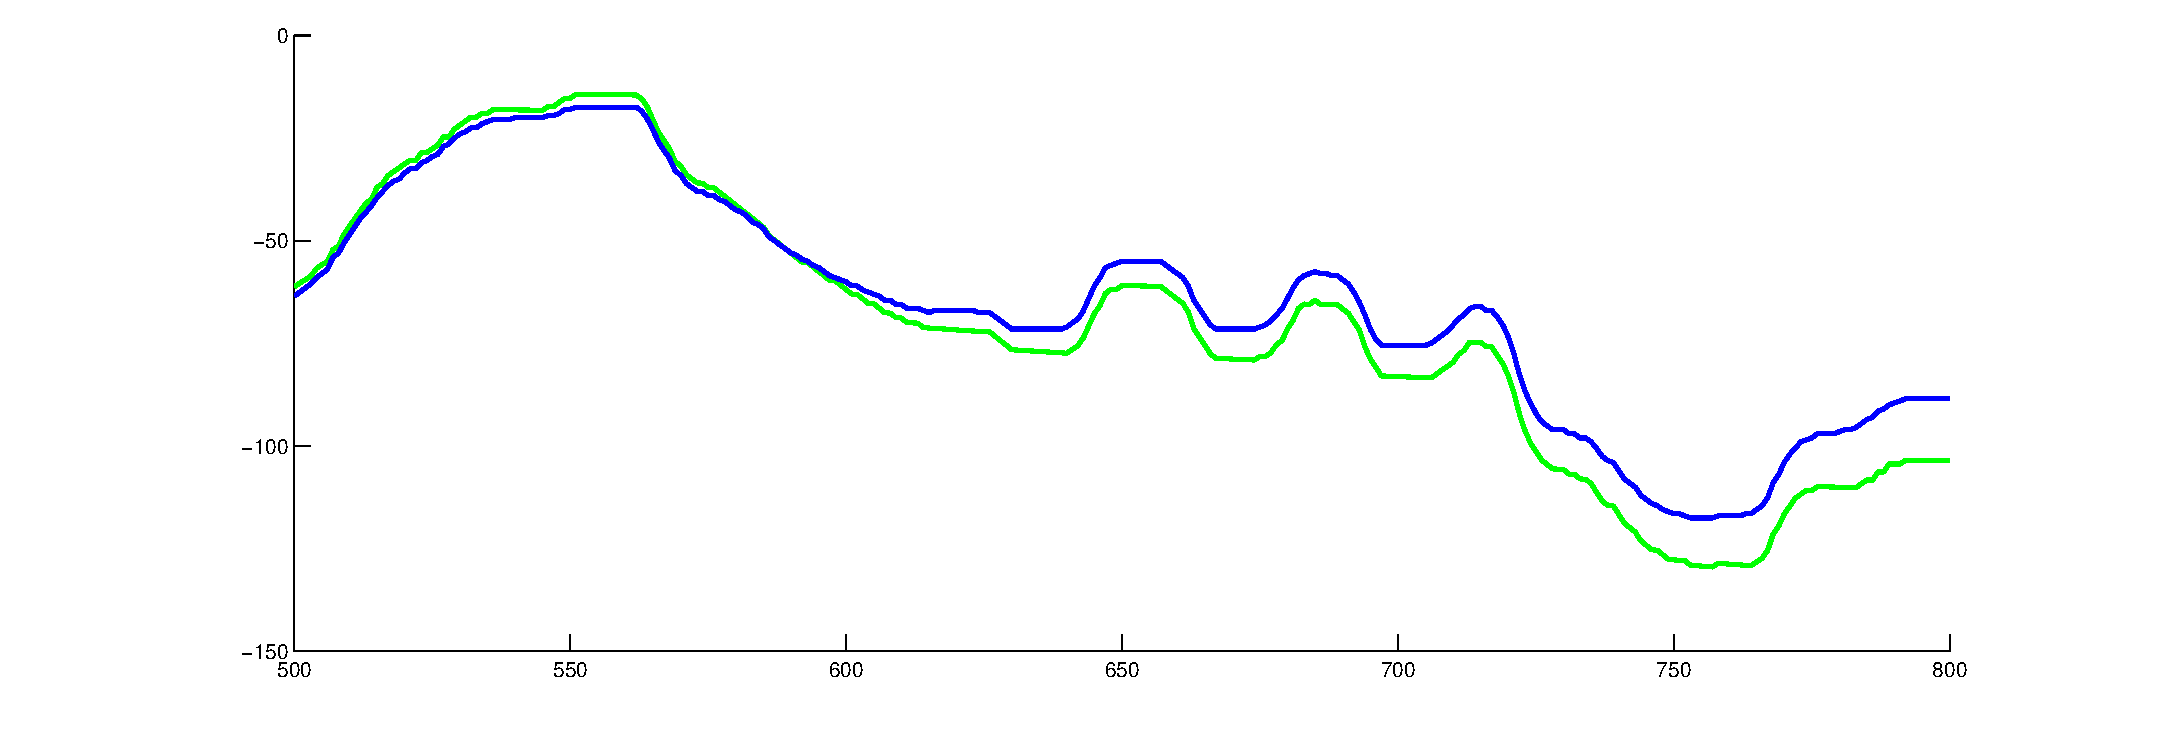
\includegraphics[width=1.0\linewidth]{images/jobbTacho.eps}
	\end{center}
	\caption{Jobb motor fordulatszám összehasonlítása a bal és jobb motor fordulatszám átlagával}
	\label{jobbTachoFig}
\end{figure}

A szinkronizálás helyességének tesztelése után, a PID szabályzó bemeneti hibáját meghatározó négy komponensnek a kiszámítását teszteltük. Gilyen Hunor által készített algoritmus esetében a robot sebességének és pozíciójának kiszámításakor átlagolva volt a két motor fordulatszáma. Esetünkben ez módosult és elhagytuk az átlagolást. Ennek eredményeként amikor egy adott iterációban minimális különbség lépet fel a két motor fordulatszáma között akkor ez nagymértékben befolyásolta sebesség és pozíció kiszámítását. Mivel a fordulatszám különbözött ezért a sebesség és a pozíció is. E különbség iterációnként növekedett. A sebesség és a pozíció a PID bementi hibájának a két komponense ezért a kimeneti érték is különbözött, amely meghatározta a motorokra adott erő nagyságát. Tehát a motorok által leadott erő különbözött és ezért a robot elvesztette egyensúlyát.

E probléma megoldására próbáltuk súlyozni az aktuális és az azelőtti mért fordulatszámot, hogy megközelítsük az átlagolt fordulatszámot. Az így megkapott értékel számoltuk ki a robot sebességét és pozícióját. A legjobb megközelítését, amelyet az átlagolt értékkel hasonlítottunk össze az látható a \ref{balTachoFig} és a \ref{jobbTachoFig} ábrákon. A kék szín jelöli a adott motor fordulatszámát illetve a zöld jelöli a motorok az átlagolt fordulatszámot. De még ez a közelítés sem volt elegendő, hogy a robot ne veszítse el az egyensúlyát.







 
